\chapter[Parameters]{Computing Bid Price Parameters}
\label{AppendixParemeters}

% \section{Relating the bid price parameters to the code}
The bid price is: 
\begin{align}
P^{bid} \ge   \frac{\phi \mathcal{R}}{(1-m)r^{target}-\left[ \delta(1+L(P)- (1+r)m)\right]}. 
\end{align}
In the following sections, we discuss each of the terms and how they are implemented in the code. Sections are numbered: 
\begin{align}
\frac{\ref{SS:rentshare}*\ref{SS:NetRent}} {(1-\ref{SS:BorrowingRatio})\ref{SS:targetr}-
\left[ \ref{SS:discountfactor}(1+\ref{SS:PriceForecast}- (1+\ref{SS:BankRate})\ref{SS:YWealthConstraint})\right]} \nonumber
\end{align}

%. \label{SS:}
\section{Rent share}\label{SS:rentshare}

a fraction
$\phi = rent-taxes-costs /rent$ 

\subsection{Target interest rate}\label{SS:targetr}

 The target interest rate, $r^{target}$, is the prime rate plus a margin. % required by the bank.  Question: do non-bank actors have such a term?

\begin{verbatim}
self.get-target-interest-rate(buyer)
\end{verbatim}

\subsection{Net rent}\label{SS:NetRent}

There's a distinction between the warranted rent, the net rent, and the rent that's actually charged.



We assume that the  rent  actually charged to a tenant is the warranted economic rent, ($\mathcal{R}= \omega - \tau d_j$), but the relevant term to enter into the calculation of return on investment is the net rent $\mathcal{R}_N$ for a given property, because the returns are the returns an investor can get after paying taxes and operating costs.

In our computational model, we do the calculation in terms of a mortgage, so we want the total returns after expenses, in present value, compounded over the mortgage  period.
% We want the total returns after expenses, in present value, compounded over a 5 year period.


\begin{align}
\mathcal{R}_N &= \mathcal{R} - \Theta - \Sigma 
\end{align}


In terms of the warranted rent, 
\begin{align}
\mathcal{R}_N &= (1-\kappa_j - \sigma_j)(\omega - \tau d_j)
\end{align}

% $\mathcal{R}_N = (1-\kappa_j - \sigma_j) (\omega - \tau d_j)$

{\color{red}
Notice that  we need here is really the fraction of the warranted rent that the owner gets to keep after maintenance costs and taxes. It is possible that the owner is charging more or less than the economic  rent, but economic rent can be seen as an equilibrium value. Economic rent is $\mathcal{R}$.  This is (tautologically) related to the price as a fraction of the actual sale price: COULD MOVE TO THE CHAPTER NOW SINCE THE THE SECTION IS MOVED THER
}

\[\mathcal{R}= \frac{\mathcal{R}}{P_0}P_0 \]

***

If we want to know the  present value  of the \textbf{net rent}, $\mathcal{R}_N$, we collect over the period  $\mathcal{R}_N^T$, we \textbf{add up} the rents each year. We assume the rents are rising and collected at the end of the year and the first is the current warranted rent.
\[\mathcal{R}_N^T= (\omega-\tau*d)\sum_{t=0}^{t=T-1} \frac{(1+\dot{\mathcal{R}})^{t}} {(1+r_{r_\delta})^{t+1}} \]

% \[\mathcal{R}_Nj^T= (\omega-\tau*d_j)\sum_{\tau=0}^{\tau=T-1}\left[\frac{1+\dot{\mathcal{R}}}{1+r_{r_\delta}}\right]^\tau \]
\noindent where $\dot{\mathcal{R}}$ is an expected rate of change of rents - possibly zero for now, and $r_\delta$ is the individual's discount rate.

TODO: problem - how to handle subscripts with net rent $\mathcal{R}_N$

\subsection{Tax ratio}\label{SS:taxratio} 
The tax ratio $\sigma$ is the share of rents that the municipality takes for services and infrastructure. Perhaps about 30\% based on mill rates in Ontario,  so $\sigma = 0.3$. % REFERENCE

*** CHECK Total taxes paid on a given property, over a given mortgage period, is $\Sigma_j = \sigma * P_j$.


\subsection{Cost tax ratio}\label{SS:costratio} 
The value of $\kappa$  varies for every property based on maintenance requirements, historic rents, tenant rights, and variations in assessed values. If it varies, it may be useful as a quality indicator.

Values for $\kappa$ and $\sigma$ must be adjusted to take into account the length of the period or net rents have to be summed over the period.


\subsection{Discount factor}\label{SS:discountfactor}

The discount factor $\delta_i$ for period $T$ captures the cost of waiting $T$ periods to sell the property. The usual; way to treat it, which we use here, is to assume that $i$ has an interest rate $r_i$ and has been investing efficiently. This means that  the individual has a discount factor for future returns base on the year-over-year rate of return. 

\[\delta_i=\left[\frac{1}{1+r_i}\right]^T\]


\subsection{Price forecast approximation} \label{SS:PriceForecast}
$L(p)$

$p$ is all the price data plus any exogenous information (EG Policy knowledge?). $L(p)$ is an estimation function that produces a `common knowledge' value for the rate of price increase. Later you can add idiosyncratic extra knowledge or extra ignorance.




\subsection{Computing the bank's interest rate}\label{SS:BankRate}
$r$

The bank's interest rate, $r$, is just the bank rate (prime rate? set by the Bank of Canada. Exogenous. Just assign  a value like 4\%.


\subsection{Computing the borrowing ratio}\label{SS:BorrowingRatio}
$m_i$

The borrowing ratio, $m_i$, is just the fraction of the price that the bank will lend to a potential buyer. \textbf{It may depend on the individual.} 

Income(\ref{SS:YWealthConstraint}) and/or wealth (\ref {SS:MWealthConstraint}) may constrain individual participation in markets. 
Here we should use the same logic as we use about the interest rate charged. (\ref{SS:BorowingRate})


It is likely to be higher for institutional buyers  and for rich people because the bank thinks rich people are more secure risks. they may have other assets that could be attached in the case of default.

\subsection{Wealth constraint on m} \label{SS:MWealthConstraint}


I have suggested that the availability of  capital is known to differ for rich and poor. 
The bank, as a person has lots of assets, so $m_i$ is close to one, say 0.9. 

For the median wealth holder, $m_i$ should be around - let's say, 0.8 and  
We need a function that captures this relationship so we need to define individual wealth:
\[W_i= P_i -M_i  +S_i\]
where 

\begin{tabular}{ll}
$P_i$ & value of owned home\\
$M_i$ & Mortgage on owned home\\
$S_i$ & personal savings = $age*d*W$\\
\end{tabular}


We first tie the borrowing \textbf{ratio}, $m_i$,  for agent $i$, to individual wealth. Figure~\ref{Fig:Borrowingratio} illustrates a mortgage availability  model that is written 
 \[ m_i = 0.1(9-\left(\frac{W_i}{\bar W}\right)^{0.5}/2 )\]
Where $\bar{W}$ is mean wealth and $W_i$ is individual wealth. 

\begin{figure}[htb]
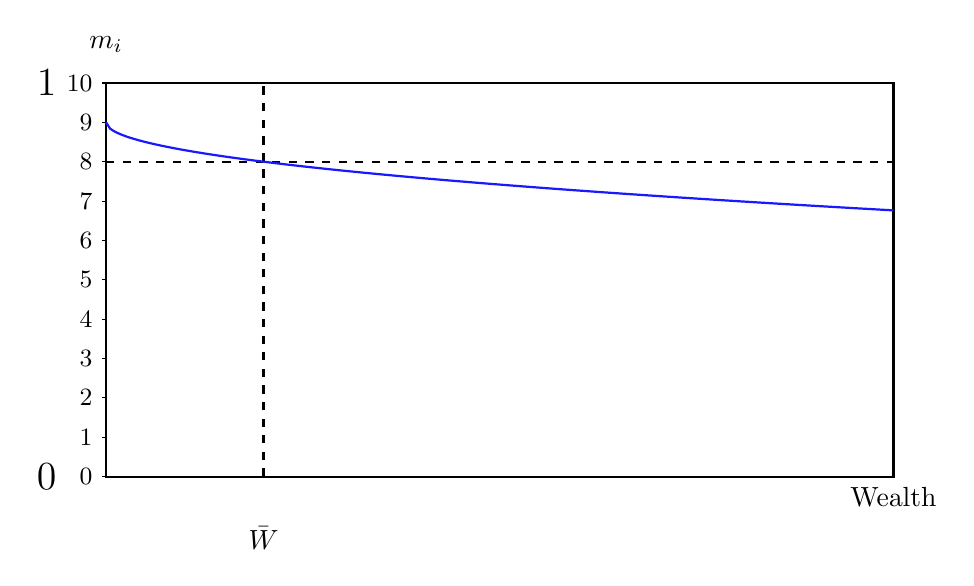
\begin{tikzpicture}[scale=.5]
%\def\bndmax{5}        %https://tex.stackexchange.com/questions/68462/filling-a-complex-region-with-tikz
%\def\bndmin{0.2}
\def\Y{10}  % height of y axis pecent
\def\W{20}  % length  of x axis
\def\Wbar{4}
\def\rbar{8}% this is the prime rate

% %Equation   \[ r_i = (A + .5 \frac{\bar{W}}{W_i})\omega\]
   % \def\Wmin{.63}  %This sets the lower limit fo the 
    \def\Wmin{(\B*\Wbar)/(\Y/\rbar-\A)} %function to keep in in bounds
	
 \tikzset{func/.style={thick,color=blue!90}}	

 \draw [thick](\W,\Y)-- (0,\Y)node[left=.5cm]{\Large$1$}node[above=.25cm]{$m_i$} -- (0,0)node[left=.5cm]{\Large$0$}--(\W,0)node[below]{Wealth}--cycle;  	% Axes box
 
 \draw [dashed, thick] (0,\rbar) -- (\W,\rbar);  	% Axes
\draw [thick,dashed] ( \Wbar,0)node[below=.5cm]{$\bar{W}$} -- (\Wbar,\Y);  	% Axes

\foreach \yi in {0,...,\Y} \draw (0,\yi)--(-.1,\yi)node[left]{\small$\yi$};
%\foreach \yi in {0,2,4,6,8,10} \draw (0,\yi)--(-.1,\yi));
%node[left]{\small$\yi$};
%\foreach \yi in {0,2,4,6,8,10}node at (-.1,yi) {{10*yi}} ;
\draw[func,domain=0:\W] plot [samples=200] (\x,(9-\x^.5/2);

 \end{tikzpicture}
\caption{Individual borrowing ratio $m_i$ as a function of wealth (in tenths)}
 \label{Fig:Borrowingratio}
\end{figure}


\subsection{Individualized borrowing rates}\label{SS:BorowingRate}
 $r_i$ 
 
 $r_i$ should depend on  both the person's income and their assets compared to others. The median after-tax income of Canadian families and unattached individuals was \$66,800 in 2020 according to Statistics Canada's \href{https://www150.statcan.gc.ca/n1/daily-quotidien/220323/dq220323a-eng.htm}{Canadian Income Survey, 2020}.  \href{https://www150.statcan.gc.ca/t1/tbl1/en/tv.action?pid=1110005501}{Data released in 2020 by Statistics Canada} indicates that the top 1\% of Canadians made, on average, around \$512,000 in a single year. \href{https://www150.statcan.gc.ca/n1/daily-quotidien/201222/dq201222b-eng.htm}{Survey of Financial Security, 2019}.

 A study by Statistics Canada found that the typical Canadian household now has a median net worth of \$329,900, while the average net worth in Canada is \$738,200. \href{https://www150.statcan.gc.ca/t1/tbl1/en/tv.action?pid=1110005501}{High income tax filers in Canada}

\subsection{Computing the income constraint on interest rates}\label{SS:YWealthConstraint}
$r_i$

In our model, we  tie the individual cost of capital,  $r_i$ for agent $i$, to a prime rate, $\bar r$ or the bank's target rate, $r^{target}$, prime plus 1\%, say. and to individual wealth. Figures~\ref{Fig:Borrowingrate1} and ref{Fig:Borrowingrate1} illustrate a couple of possible  cost-of-borrowing models roughly consistent  with the stylized facts about lenders. 

\begin{align}
 r_i =  &  \left(A + B \frac{\bar{W}}{W_i}\right) \bar r       \label{eq:incomeandr1}  \\
 r_i =  &  \left(\bar r - A + B *\frac{\bar W}{W_i - C}\right) \label{eq:incomeandr2}  \\
\end{align}
Where $\Bar{W}$ is mean wealth and $W_i$ is individual wealth. In Equation~\ref{eq:incomeandr2},  A determines y-shift, B, the scale, and C the  x-shift for the curve.


\begin{figure}
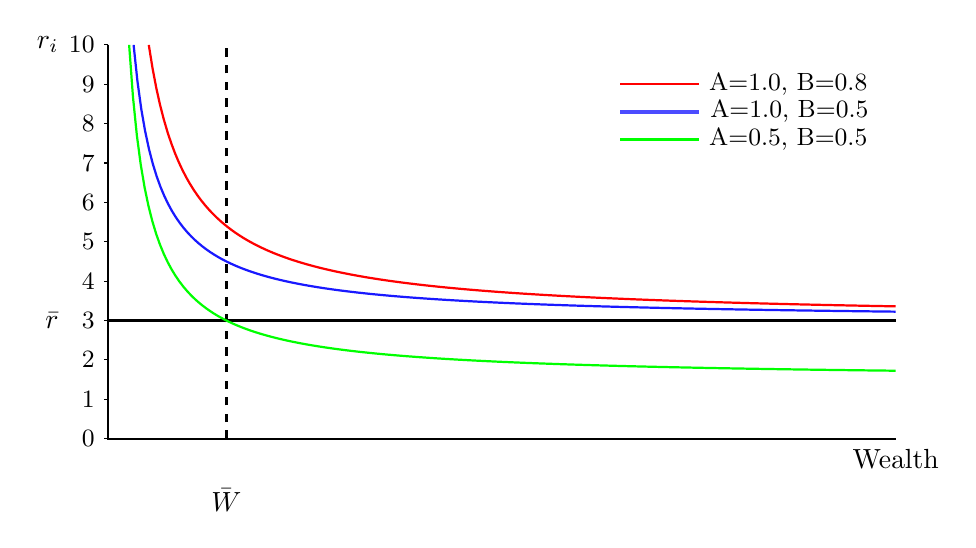
\begin{tikzpicture}[scale=.5]
%\def\bndmax{5} % https://tex.stackexchange.com/questions/68462/filling-a-complex-region-with-tikz
%\def\bndmin{0.2}
\def \Y {10}    % height of y axis as a pecent
\def \W {20}    % length  of x axis
\def \Wbar {3}  % mean wealth
\def \rbar {3}  % the prime rate 

% Equation   \[ r_i = (A + .5 \frac{\bar{W}}{W_i})\omega\]
\def \Wmin{.63}  %This sets the lower limit fo the 
\def \Wmin{(\B*\Wbar)/(\Y/\rbar-\A)} %function to keep in in bounds
\tikzset{func/.style={thick}}	

% Axes
\draw [thick] (0,\Y)node[left=.5cm]{$r_i$} -- (0,0)--(\W,0)node[below]{Wealth};  
\foreach \yi in {0,...,\Y} \draw (0,\yi)--(-.1,\yi)node[left]{\small$\yi$};
\draw [thick] (0,\rbar)node[left=.5cm]{$\bar r$} -- (\W,\rbar);  	% Axes
\draw [thick,dashed] ( \Wbar,0)node[below=.5cm]{$\bar{W}$} -- (\Wbar,\Y);  	% 

\def \A {1.0}  \def \B {0.5} %BLUE
\draw[func,domain=\Wmin:\W, color=blue!90] plot [samples=200] (\x,{(\A+\B*\Wbar/\x)*\rbar});
\draw [ultra thick, color=blue!70 ](13, 8.3)--(15,8.3)node [right, black] {\small A=\A,\ B=\B};

\def \A {0.5} 
\def \B {0.5} % GREEN
\draw[func,domain=\Wmin:\W, color=green] plot [samples=200] (\x,{(\A+\B*\Wbar/\x)*\rbar});
\draw [thick,  color=green](13, 7.6)--(15,7.6)node [right, black] {\small A=\A, B=\B};

\def \A {1.0}  \def \B {0.8} % RED
\draw[func,domain=\Wmin:\W, red] plot [samples=200] (\x,{(\A+\B*\Wbar/\x)*\rbar});
\draw [thick,  color=red](13, 9)--(15,9)node [right, black] {\small A=\A,\ B=\B};
% KEY
\end{tikzpicture}
\caption{Individual borrowing cost as a function of wealth}
\label{Fig:Borrowingrate1}
\end{figure}


\begin{figure}
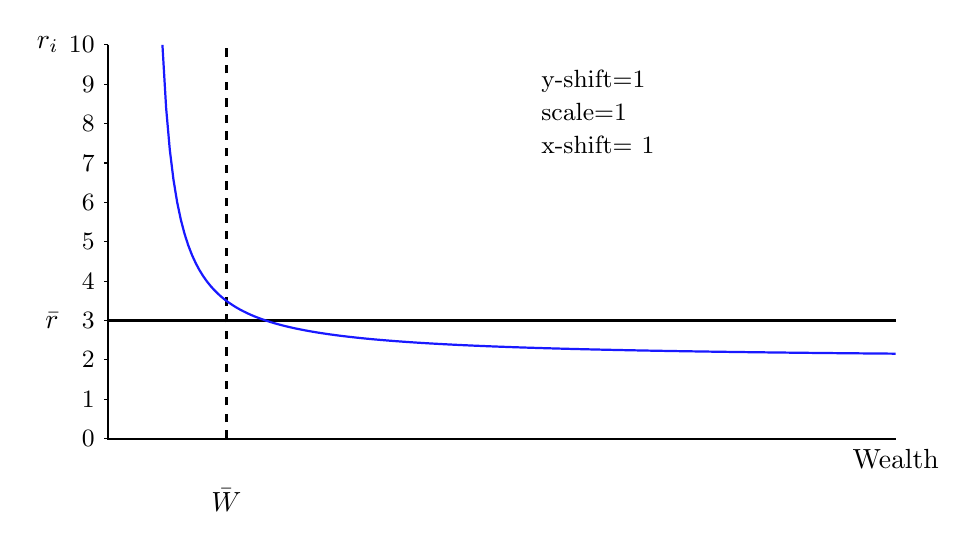
\begin{tikzpicture}[scale=.5]
%\def\bndmax{5}        %https://tex.stackexchange.com/questions/68462/filling-a-complex-region-with-tikz
%\def\bndmin{0.2}
\def \Y {10}  % height of y axis pecent
\def \W {20}  % length  of x axis
\def \Wbar {3} % meam wealth
\def \rbar {3}% this is the prime rate 

%\def \Wmin{(\B*\Wbar)/(\Y/\rbar-\A)} %function to keep in in bounds
\tikzset{func/.style={thick}}	
	% Axes
\draw [thick] (0,\Y)node[left=.5cm]{$r_i$} -- (0,0)--(\W,0)node[below]{Wealth};  
\foreach \yi in {0,...,\Y} \draw (0,\yi)--(-.1,\yi)node[left]{\small$\yi$};
\draw [thick] (0,\rbar)node[left=.5cm]{$\bar r$} -- (\W,\rbar);  	% Axes
\draw [thick,dashed] ( \Wbar,0)node[below=.5cm]{$\bar{W}$} -- (\Wbar,\Y);  	% 

\def \A {1} %vertical shift aroung \rbar, the prime rate
 \def \B {1}  % Scales the exponential curveBLUE
 \def \C {1}  %right shift  
% \def \Wmin {.4+\B}  %This sets the lower limit fo the 
\def \Wmin {(\B*\Wbar)/(\Y-\rbar+\A) +\C} %function to keep in in bounds

\draw[func,domain=\Wmin:\W, color=blue!90] plot [samples=200] (\x,{\rbar-\A+\B*\Wbar/(\x-\C))});
\node  [align=left, text width =2cm ] at (13, 8.3) {\small y-shift=\A \newline scale=\B \newline x-shift= \C};

 \end{tikzpicture}
\caption{Individual borrowing cost as a function of wealth II}
\label{Fig:Borrowingrate2}
\end{figure}

The rates $\delta,\ \sigma,$ and $r$ depend on the period, $T$. 

\section{Incorporating growth and discounting}
%We need a time period T for calculations. For use in any calculation, 

With a price-growth rate of $\dot P$ per year, the growth over $T$ years is $(1+\dot P)^T$, and  %and a 5 year mortgage period, 
the expected price at the end of the period is:

\[P^e_T=P_0(1+\dot P)^T\]

If, for example price growth is 10\%, $\dot P= 0.1$, the {capital gain}, or growth, over a 5-year mortgage term is 0.61051 $\approx$ 60\% of the original price, $P_0$.

If we want the compounded interest rate person $i$ the term T,
\[r_i^T=(1+r_i)^T\]
% This is the value we use in equation~\ref{EqBidPrice}.

If person $i$  discounts at a discount rate $r^\delta$, the present value of a receipt at time $t$ is calculated by using the \textbf{discount factor} $\delta_i^T$.

\[\delta_i^T= \left( \frac{1}{1+r_\delta} \right)^T \]
%\[\delta_i^T= \sum_{\tau=0}^{\tau=T}\left( \frac{1}{1+r_\delta} \right)^\tau \]
 
These can be combined into a function %\delta that  gives a single discounting factor  for a value  like future price that is both growing and being discounted over several (T) periods:
\[ PDV(P^e_T)=P_0\left( \frac{1+\dot P}{1+r_\delta} \right)^T \]
This PDV function specifically combines any expected rent increase, the individual's discount rate and the mortgage term into a single operation.

\subsection{Mortgage availability}
For home loans, many personal finance experts recommend total housing costs account for less than 28\% of your \textbf{gross} household income, This gives us an \textbf{income-based  mortgage maximum} of \[M^{max}_Yi = \frac{0.28*(\omega+w)}{r_i}\] It is the maximum the bank will let you pay.

We assume $r_i$ is based on the individual's assets, on relative wealth. Where is it calculated for the householder or the bank?

We get a \textbf{price-based mortgage maximum} \[M^{max}_P = 0.8P_0\] where $P_0$ is the actual sale price. This is based on the maximum amount of risk that the bank is willing to take on. ($P_0$  will not always be the same as the asking price or the warranted price.)


\section{Table}

\renewcommand{\arraystretch}{1.5}
\begin{tabular}{rlrr}\
Symbol         & Name                                 & Value      & Formula  \\ \hline
$m_i$          & Individual borrowing-ratio           & 0.75-0.85  & $M/P^{ask?}$ \\
$M^{max}_Yi$.  & Maximum mortgage based on income     &            & $\frac{0.28(\omega+w)}{r_i}$ \\
 $M^{max}_P$   & Maximum mortgage based on the price  &            & $0.8*P_0$ \\
$IS$           & Income share for housing debt        & 0.25-0.35  & Missing? \\
$\rho$         & Rent ratio                           &            & $\frac{\omega-tau*d_i}{P_0}$ \\
$\kappa $      & Operations ratio                     & 0.1-0.3    & e.g. $ 0.2\frac{\omega-tau*d_i}{P_0}$ \\
$\sigma$       & Tax ratio                            & 0.25-0.35  & e.g. $ 0.3\frac{\omega-tau*d_i}{P_0}$ \\
$\dot P $      & Price growth                         & []         & $\frac{P_t-P_{t-1}}{P_{t-1}}$\\
$P^T_e$        & Expected price in T years            &            & $P_0(1+\dot P)^T$ \\ % *** WAS $P^e_T$ 
$r_i^\delta$   & Individual discount rate             &            & To assign \\
$\bar r$       & Prime interest rate                  &            & \\
$r_i$          & Individual borrowing-rate            &            & \\
$r^{target}$   & Target interest rate                 &            & $\bar r + margin$ \\
$\delta_i$     & Discount factor for T                &            & $\left(\frac{1}{1+r_i^\delta}\right)^T$ \\
\end{tabular}
\renewcommand{\arraystretch}{1.0}


todo look for $P^e_T$ 

%==========================EXAMPLE=========================== https://www.kaggle.com/code/prateekmaj21/basic-financial-calculations-using-python/notebook
  
% def compound_interest(p,r,t):  %EXAMPLE
    
%     print('Amount: ', p)
%     print("Rate of Interest (Per Annum)", r)
%     print("Time (In Years): ",t)
    
%     a= p*((1+r/100)**t)
    
%     ci= a-p
%     print("Final Amount: ", a)
%     print("Compound Interest: ", ci)
 

\section{Transportation costs}
Transport costs have two parts:
1) fuel and vehicle costs per km
2) time costs per km

\subsection{Vehicle related costs}
Use one year as the wage period, converting transportation costs per km to annual cost for consideration in the household budget. Starting with the cost per km, calculate the cost per year:

\textbf{cost per km =$\textit{t}$}:. \$0.59   (from  Ontario data, 2021). sensitive to congestion, use of subways (\$5 /day?), 

 \textbf{work trips per year} 2 way * 5 days/week * 50 weeks work days = 500. [range: 450-550]

\textbf{cost per km-year} = work trips per year*cost per km

=\$0.59/km*500 trips/year  =  \$295/km year 



\subsection{Time costs}
\textbf{time per km}. range: 20km/hr -> 3min/km, 40km/hr -> (1.5min/km - 3min/ km)per trip 

(New York rush hour is much slower:  4-9km/hr ->6-15 min/km)

\textbf{time  per km-year} = work trips per year*time t per trip = 500* 3min  = 1500 min/km year = 25 hours= 3-3.5 days/km
 
\textbf{time cost per km-year} =  (days per km-year /work days/year)*wage premium per year  = 3/250 = 0.012 years/km year. ?

\textbf{money cost of time per km year} 

=time cost per km-year* wage(including subsistence) 

= 0.012 year* wage per year

\subsection{Total cost per km year of commuting for one agent}
\textbf{money cost of time per km year + \$295/km year * distance} \\
= (0.012 w+ \$295)/km year 
    \begin{quotation}
    \textbf{Example}
    To get a sense of the required wage if we have this annual cost structure, assume city\_extent $d^*$ is 30 km. At this point the transport cost is equal to the wage

\[(0.012 w+ \$295)/km year)*30 =  w\] 
\[.36w+ 8850=w\]
\[w=13828.12\]
        \begin{quotation}
        \textbf{PLAUSIBILITY CHECK}
This is plausible land rent, but does not include building rent. 
Capitalized at 5\% this house is worth \$ 276,562, a fairly cheap house 30 miles from city centre
        \end{quotation}
    \end{quotation}

{\color{red}
\subsection{? Value of $t$ to use in model}}
\[ \tau=(0.012 w+ \$295)/km year \]

